\chapter{مروری بر کارهای گذشته در شرایط کنترل نشده}
\section{مقدمه}
در سال های اخیر روش های تشخیص چهره بسیار زیادی به منظور یافتن و شناسایی چهره افراد در تصویر پیشنهاد شده است که توانایی مقاومت در برابر مشکلات و چالش های رایج مانند تغییرات شدید روشنایی، تغییر حالت و زاویه چهره، انسداد ، تاری خارج از تمرکز، سالخوردگی و... را ندارند و در کاربردهایی نظیر شرایط کنترل نشده قابل استفاده نیستند. در بخش مقدمه در مورد چالش های موجود در فرایند تشخیص چهره صحبت شد. برای رفع این چالش ها و بهبود طبقه بندی، راه حل هایی پیشنهاد شده است که در این بخش مورد بررسی قرار گرفته اند.
جدول \ref{table3-1} خلاصه ای از روش های مقابله با شرایط کنترل نشده

\begin{table}[ht]
\label{table3-1}
\begin{center}
\resizebox{\textwidth}{!}
{
\begin{tabular}{|c|c|c|c|c|}
\hline 
مقاله ها & چالش مورد نظر & رویکرد & مزیت ها & مشکل ها
\\
\hline 
\cite{HAGHIGHAT201623, LV2016465, amos2016openface, 6196234}
& حالت چهره	 & تبدیل دوبعدی & 	پیچیدگی محاسباتی قابل قبول & 	استخراج نقاط ویژه باید دقیق تر باشد
 \\
\hline
\cite{wu2016facial, 7477555, 7780892, 7532959, 7298667}
 & حالت چهره & 	استفاده از شبکه عصبی عمیق & دقت بالا در شرایط کنترل نشده & 	پیچیدگی محاسباتی، وابستگی به داده های آموزش 
\\
\hline
\cite{HU2017366, hassner2014effective, 7298679, 7006757, 6905796}
 & حالت چهره & 	تبدیل مدل دو بعدی به سه بعدی & 	دقت بالا 	پیچیدگی محاسباتی &
\\
\hline 
\cite{DING2017144}
& حالت چهره & 	تبدیل مدل سه بعدی به دو بعدی & 	دقت بالا 	پیچیدگی محاسباتی &
\\
\hline
\cite{6196234, HUSSAINSHAH201597}
 & روشنایی	 & همسان سازی بافت-نگار & 	پیچیدگی محاسباتی قابل قبول & 	قابل استفاده در تصاویر خاکستری
\\
\hline
\cite{7015448, WU2018256}
 & انسداد	 & استفاده از روش های شناسایی الگو و وایازش & 	دقت بالا در انسداد شدید &	
\\
\hline
\cite{7984553}
 & محدودیت داده	 & تهیه مجموعه داده با ردیابی چهره در ویدیو & 	تهیه مجموعه داده با دقت بالا & 	نیاز به یک مرحله طولانی استفاده از تصاویر ویدیو
\\
\hline
\cite{6249269, HU2018582}
 & محدودیت منابع & 	استفاده از رایانش ابری & 	سرعت بالا & 	تجهیزات پیشرفته و زمان تاخیر ناهمگن
\\
\hline
\end{tabular}}
\end{center} 
\end{table} 

\section{چالش حالت}
چالش حالت زمانی پیش می آید که چهره فرد کاملا رو به روی دوربین قرار نگیرد و دارای زاویه زیادی باشد. در این شرایط با توجه به ساختار سه بعدی چهره، ممکن است سامانه نتواند ویژگی های درستی از چهره استخراج نماید و در تشخیص هویت دچار اشتباه شود. گرچه شبکه عصبی پیچشی توانایی مقابله با این چالش را از طریق استفاده از مجموعه داده های بزرگ و آموزش تصاویر مختلف از حالات چهره دارد، اما این کار باعث بزرگ شدن پایگاه داده و کند شدن سامانه می‌شود. استفاده از یک پی برنده \LTRfootnote{Heuristic} به منظور کاهش حجم داده های آموزش می تواند نتایج بهتری به دنبال داشته باشد. یکی از راه  حل های مقابله با این چالش، هنجار سازی، رو به رو سازی \LTRfootnote{Frontalization} و هم ترازی \LTRfootnote{Alignment} چهره می‌باشد. در ادامه برخی رویکردهای رو به رو سازی و هم ترازی چهره در شرایط کنترل نشده را دسته بندی می کنیم.

\begin{enumerate}
\item
رویکرد های دو بعدی با پیچیدگی محاسباتی قابل قبول (بیشتر ایده های مبتنی بر نشانه گذاری \LTRfootnote{Landmark} قدیمی) مانند 
\cite{HAGHIGHAT201623, LV2016465, amos2016openface, 6196234}.

\noindent
مشکل: در محیط های بدون محدودیت مانند آنچه که در این پروژه داریم، استخراج دقیق مکان نشانه های صورت از تصاویر دو بعدی نیاز به توجه بیشتری دارد. پیشرفت های اخیر مانند \cite{HAGHIGHAT201623} است.

\noindent
مزیت: این الگوریتم ها از نظر پیچیدگی محاسباتی \LTRfootnote{Computational Complexity} قابل قبول هستند و کاملا برای شرایط این پروژه متناسب می‌باشند.
\item 
رویکردهای مبتنی بر شبکه عصبی برای تخمین و اصلاح موقعیت چهره (آموزش و آزمایش با تصاویر دو بعدی) مانند 
\cite{wu2016facial, 7477555, 7780892, 7532959, 7298667}.

\noindent
مشکل: این الگوریتم ها، به طور متوسط، کندتر از دسته پیشین می‌باشند. اما بستگی به این دارد که عمق شبکه عصبی چه مقدار باشد. وابستگی آن ها به داده های آموزش می‌باشد و مراحل مجزای رو به رو سازی و هم ترازی چهره ندارند.

\noindent
مزیت: بدون نیاز به تصمیم گیری در مورد مجموعه بهینه ای از نشانه های چهره و دارای دقت بیشتر در شرایط کنترل نشده با انسداد و... . ایده هایی مانند \cite{Martino2015} برای تخمین موقعیت چهره ممکن است به زمان محاسبات کمک کند.
\item

رویکردهای سبک سه بعدی بدست آمده از تصاویر دو بعدی، مانند 
\cite{HU2017366, hassner2014effective, 7298679, 7006757, 6905796}.

\noindent
مشکل: زمان محاسباتی بالا. یکی از امیدوار کننده ترین این الگوریتم ها در مورد پیچیدگی محاسباتی، \cite{hassner2014effective} است که در شرایط بدون محدودیت آموزش دیده و آزمایش شده است. شامل مراحل مجزای رو به رو سازی و تراز بندی چهره می-باشند، اما برای محدودیت های این پروژه قابل استفاده نمی‌باشند.

\noindent
مزیت: با استفاده از اطلاعات سه بعدی، این روش ها به بالاترین دقت تصمیم گیری در میان سه نفر رسید.
\item
رویکرد های تبدیل مدل سه بعدی چهره به مدل دو بعدی چهره (روش های مبتنی بر پنجره \LTRfootnote{Patch-Based} بر اساس چند نمایش دو بعدی مختلف از چهره) مانند \cite{DING2017144}
\noindent
مشکل: زمان محاسباتی (نه به اندازه الگوریتم های دسته سوم). 

\noindent
مزیت: عملکرد بهتر در رو به رو سازی چهره در شرایط کنترل نشده نسبت به الگوریتم های دسته اول. ممکن است برای شرایط این پروژه متناسب باشند.
\end{enumerate}

مرجع \cite{Masi2018DeepFR} در سال 2018 خلاصه ای از رویکردهای مختلف برای حل مسئله هم ترازی را در شکل \ref{image3-1} نشان داده است. تصویر سمت چپ، چهره ورودی می‌باشد. \lr{(a)} هم ترازی با استفاده از تبدیلات دو بعدی ساده می‌باشد. \lr{(b)} داده افزایی \LTRfootnote{Data Augmentation} با تغییر مقیاس، تغییر زاویه و جا به جایی می‌باشد. \lr{(c)} برش های چندگانه می‌باشد. \lr{(d)} داده افزایی مبتنی بر روش های سه بعدی می‌باشد. \lr{(e)} از هیچ ابزاری برای هم ترازی مستقیم استفاده نمی‌نماید. اما یک شبکه را آموزش می دهد تا عامل‌های مورد نیاز برای تبدیل هم ترازی را بدست آورد.

\begin{figure}[h]
\centering
  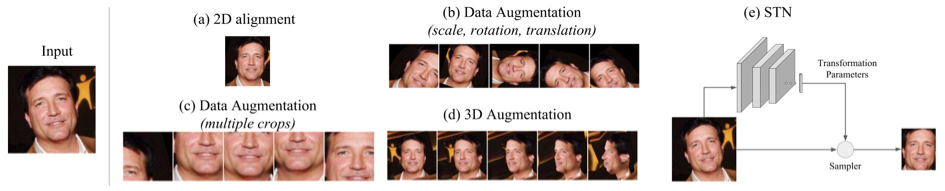
\includegraphics[scale=1]{image3-1}
  \caption{رویکردهای مختلف هم ترازی چهره \cite{Masi2018DeepFR}.}
  \label{image3-1}
\end{figure}

\noindent
در سال 2016، \lr{Brandon Amos} و همکاران در \cite{amos2016openface} یک روش شناسایی چهره به نام \lr{OpenFace} ارائه دادند که ویژگی اصلی آن، آموزش شبکه عصبی عمیق در کمترین زمان و قابلیت اجرا بر روی دستگاه های قابل حمل مانند تلفن همراه با در نظر گرفتن منابع محدود می‌باشد. یک تصویر شامل تعدادی چهره به الگوریتم داده می‌شود. پس از یافتن چهره‌ها و مجزا کردن \LTRfootnote{Isolate} آن‌ها از یکدیگر، هر چهره به طور جداگانه مورد پیش پردازش \LTRfootnote{Preprocessing} قرار می گیرد و حجم آن کاهش می یابد. کاهش حجم تصویر برای عملکرد مناسب یک طبقه بندی بهینه بسیار مهم می‌باشد. تصاویر چهره ها باید هنجارسازی شده و ابعاد آن ها ثابت گردد تا به بخش شناسایی چهره راه یابند. هر تصویر چهره باید مورد تبدیل قرار بگیرد تا چشم ها، بینی و دهان، در مکان مشخصی قرار گیرند. بدین منظور از یک تبدیل هم نسبی \LTRfootnote{Affine Transformation} دوبعدی ساده استفاده می گردد. ابتدا باید چهره توسط 68 نقطه ویژه، نشانه گذاری شود. سپس نشانه های اطراف چشم ها و بینی (شکل \ref{image3-2}) برای محاسبه عامل های تبدیل هم نسبی استفاده می‌شوند. پس از انجام تبدیل هم نسبی، تصاویر چهره برش زده شده و اندازه آن ها 96×96 پیکسل می‌شود.

\begin{figure}[h]
\centering
  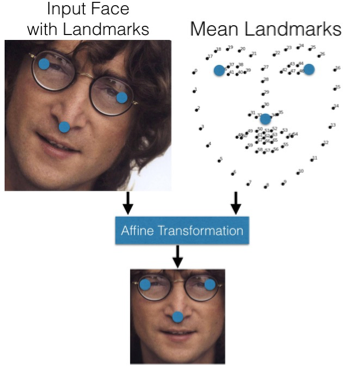
\includegraphics[scale=1]{image3-2}
  \caption{
  تبدیل هم نسبی \lr{OpenFace} براساس نقاط ویژه آبی  
  \cite{amos2016openface}.}
  \label{image3-2}
\end{figure}

\noindent‏ 
پس از پیش پردازش، تصاویر چهره ها به عنوان ورودی به یک شبکه عصبی پیچشی داده می‌شوند (شکل \ref{image3-3}). این الگوریتم برای تعلیم شبکه از مجموعه داده کوچکی با 500 هزار تصویر چهره استفاده می کند که از ادغام دو مجموعه داده بزرگ برچسب گذاری شده به نام \lr{CASIA-WebFace} و \lr{FaceScrub} بدست آمده است. شبکه مورد استفاده در این الگوریتم یک نسخه اصلاح شده از شبکه \lr{nn4} الگوریتم \lr{FaceNet} می‌باشد. شبکه \lr{nn4} مبتنی بر معماری \lr{GoogLeNet} می‌باشد. برای تعیین میزان شباهت نتیجه، از فاصله اقلیدسی استفاده شده است.
 \begin{figure}[h]
\centering
  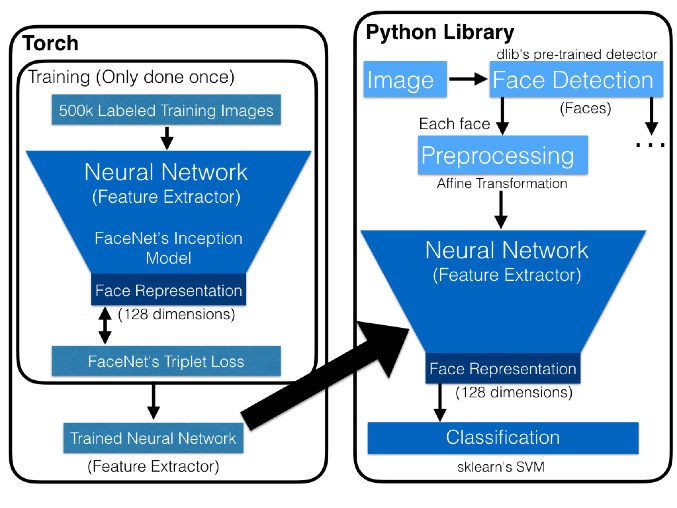
\includegraphics[scale=1]{image3-3}
  \caption{معماری \lr{OpenFace}  \cite{amos2016openface}.}
  \label{image3-3}
\end{figure}

\noindent
هر تصویر از یک شبکه یکتا به یک سه گانه نگاشت داده می‌شود. گرادیان خطای سه گانه برای هر تصویر محاسبه شده و به عقب انتشار می یابد. در هر دسته کوچک\LTRfootnote{Mini Batch}، \lr{P} تصویر برای هر نفر از \lr{Q} نفر، در مجموعه داده انتخاب می‌شود. سپس $M \approx PQ$ تصویر به شبکه داده می‌شود تا عملیات \lr{forward} انجام پذیرد. در این مقاله از $P=20$ و $Q=15$ استفاده شده است. تمام جفت های \lr{anchor-positive} برای بدست آوردن سه گانه های $N = Q \binom{P}{2}$ مورد استفاده قرار می گیرند. خطای سه گانه محاسبه شده و مشتق آن برای پس انتشار خطا استفاده می‌شود. شکل \ref{image3-4} چگونگی آموزش شبکه را نشان می دهد.

 \begin{figure}[h]
\centering
  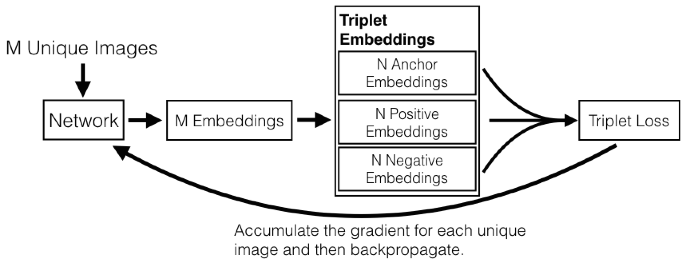
\includegraphics[scale=1]{image3-4}
  \caption{جریان یادگیری در معماری \lr{OpenFace} \cite{amos2016openface}.}
  \label{image3-4}
\end{figure}

\noindent
مجموعه داده \lr{LFW} یک معیار استاندارد برای سنجیدن میزان دقت الگوریتم های تشخیص چهره می‌باشد. الگوریتم \lr{OpenFace} بر روی این مجموعه داده مورد سنجش قرار گرفت که به دقت
 $0.9292 \pm 0.0134 \%$ 
رسید.

\noindent
در سال 2016 \lr{Mohammad Haghighat} و همکاران در \cite{HAGHIGHAT201623} یک روش برای هنجارسازی حالت چهره بر اساس تنظیم کردن مدل  ظاهری فعال \LTRfootnote{Active Appearance Model} یا \lr{AAM} ارائه دادند. \lr{AAM} یک مدل پارامتری است که برای ارائه یک شکل مانند چهره انسان استفاده می‌شود. در این الگوریتم ابتدا یک \lr{AAM} بر روی تصویر چهره قرار گرفته، با روندی تکراری و به صورت بهینه شونده، بر روی چهره تنظیم می‌شود. سپس با استفاده از یک تبدیل هم نسبی، مرحله رو به رو سازی بر روی چهره انجام می‌پذیرد. شکل \ref{image3-5} رویکرد کلی این الگوریتم را نشان می دهد. 

\begin{figure}[h]
\centering
  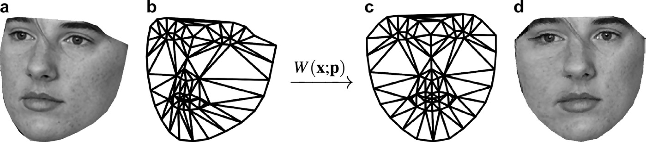
\includegraphics[scale=1]{image3-5}
  \caption{رویکرد کلی الگوریتم مبتنی بر \lr{AAM} برای رو به رو سازی چهره \cite{HAGHIGHAT201623}.}
  \label{image3-5}
\end{figure}

\noindent
در این مدل یک تصویر چهره با مجموعه ای از نقاط ویژه هنجارسازی شده مدل می‌شود که به صورت $[x_i , y_i]$ تعریف می‌شود که در آن $i=1.\ 2.\ \ldots n $. برای انجام این کار یک مرحله یادگیری نیاز است. سپس الگوریتم \lr{PCA} اعمال می‌شود تا کاهش میزان وابستگی میان نقاط ویژه در هر مجموعه انجام می‌شود و نتیجه یک مدل خطی است که یک مدل شکل نمونه را به صورت رابطه \ref{eq3-1} نمایش می‌دهد.

\begin{equation}\label{eq3-1}
S=s_0+\sum_{i=1}^{n}{p_is_i}
\end{equation}

\noindent
که در آن $s_0$ شکل پایه، $s_i$ نشان دهنده \lr{i} امین شکل پایه و [$p_1$, $p_2$, \ldots, $p_n$] عامل های شکل می‌باشند. ظاهر \LTRfootnote{Appearance} مدل \lr{AAM} یک تصویر \lr{A(x)} می‌باشد که در آن \lr{x} مجموعه پیکسل های داخل شکل پایه $s_0$ می‌باشد. مدل ظاهر یک چهره خاص از یک ظاهر پایه $a_0$ و ترکیب خطی از بردارهای ویژه
$a_i\ ,\ \ i=1.\ 2.\ \ldots m$
تشکیل می‌شود که به صورت رابطه \ref{eq3-2} تعریف می‌گردد.

\begin{equation}\label{eq3-2}
A(x)=a_0(x)+\sum_{i=1}^{m}{q_ia_i(x)}
\end{equation}

\noindent
که در آن $[q_1, q_2, \ldots , q_m]$ عامل های ظاهر می‌باشند. عامل های شکل و ظاهر برای هر تصویر در فرایند \lr{AAM} بدست می آید. الگوریتم های \lr{POIC} \LTRfootnote{Project-Out Inverse Compositional}و \lr{SIC} \LTRfootnote{Simultaneous Inverse Compositional} دو الگوریتم شناخته شده برای این منظور می‌باشند. رویکرد \lr{SIC} نسبت به \lr{POIC} در شرایطی که تصاویر آزمایشی با تصاویر آموزشی متفاوت باشند، بسیار بهتر عمل می کند. اما از طرفی دارای پیچیدگی محاسباتی بیشتری می‌باشد. در این مقاله از یک روش \lr{SIC} سریع برای حل مسئله بهینه سازی با 100 تکرار استفاده شده است. اگر $p=[p_1, p_2, \ldots , p_n]$ مجموعه عامل های بدست آمده باشد، یک تبدیل هم نسبی قطعه ای\LTRfootnote{Piecewise Affine Transformation}  \lr{W(x; p)} برای رو به رو سازی چهره مورد استفاده قرار می گیرد که در آن هریک از مثلث های روی توری، به صورت جداگانه به تصویر نتیجه با استفاده از درونیابی نزدیک ترین همسایه \LTRfootnote{Nearest Neighbor Interpolation} نگاشت پیدا می نمایند. برای مقداردهی اولیه از یک مدل پایه $s_0$ استفاده می‌شود که مقدار \lr{p} در آن صفر می‌باشد (شکل \ref{image3-6} قسمت \lr{a}). 
 \begin{figure}[h]
\centering
  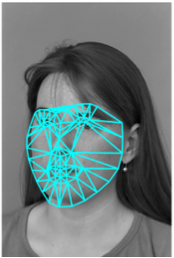
\includegraphics[scale=1]{image3-6}
  \caption{ مقدار دهی اولیه و بهینه سازی \lr{AAM} \cite{HAGHIGHAT201623}.}
  \label{image3-6}
\end{figure}

\noindent
پس از تنظیم کامل مدل بر روی چهره، یک تبدیل هم نسبی با پارامترهای بدست آمده توسط الگوریتم یادگیری یاد شده، می تواند حالت چهره را هنجارسازی نماید. در بخش شناسایی چهره، ابتدا بخش چانه از تصویر حذف می‌شود زیرا چانه تقریبا تاثیری در شناسایی یک چهره ندارد. سپس تصویر چهره به اندازه 64×64 پیکسل تبدیل می‌شود و به 64 بخش غیر هم پوشان با اندازه 8×8 تقسیم می‌شود. سپس در هر بخش تبدیل \lr{DCT} \LTRfootnote{Discrete Cosine Transform} انجام می‌شود. ضرایب خروجی تبدیل \lr{DCT} بر حسب یک پویش زیگزاگی مرتب می‌شوند. اولین ضریب در نظر گرفته نمی‌شود. زیرا نشان دهنده میانگین سطح خاکستری پیکسل های بخش می‌باشد. 10 ضریب بعدی که ضرایب فرکانس پایین می‌باشند، برای ایجاد بردار ویژگی چهره استفاده می‌شوند. برای آموزش و آزمایش از مجموعه داده \lr{FERET} و \lr{LFW} استفاده شده است که در آن تصاویر چهره با زوایای چرخش متفاوت وجود دارند. الگوریتم مورد استفاده در این مقاله موفق به دستیابی به شناسایی چهره با دقت 87.3\% شده است. در شکل \ref{image3-7} نتیجه آزمایش بر روی مجموعه داده  \lr{FERET} در زاویه های متفاوت قابل مشاهده می‌باشد.

 \begin{figure}[h]
\centering
  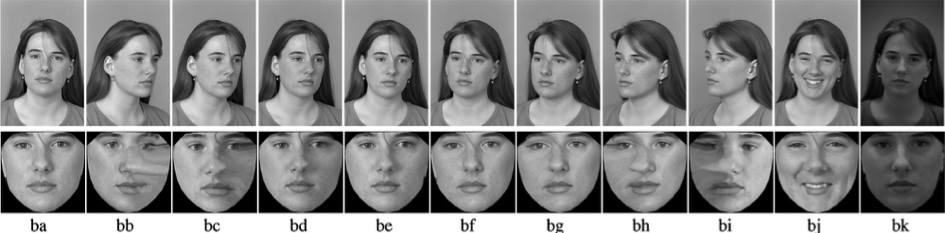
\includegraphics[width=1.0\textwidth]{image3-7}
  \caption{نتیجه آزمایش بر روی مجموعه داده  \lr{FERET} در زاویه های متفاوت \cite{HAGHIGHAT201623}.}
  \label{image3-7}
\end{figure}

\noindent
در سال 2016، \lr{Zhang} و همکاران در \cite{7532959} یک روش رو به رو سازی چهره ارائه دادند که شناسایی چهره را مستقل از نمای چهره \LTRfootnote{Facial View} انجام می دهد. این الگوریتم یادگیری عمیق که \lr{VS2VI} نامیده می‌شود، از دو بخش اصلی تشکیل شده است. بخش اول یک شبکه عصبی پیچشی برای یادگیری نما و زاویه چهره می‌باشد و بخش دوم از تعدادی شبکه عصبی پیچشی تشکیل شده است که هر کدام برای یادگیری تناظر \LTRfootnote{correspondence} بین یک چهره از رو به رو با یک چهره از یک زاویه و نمای خاص می‌باشد (شکل \ref{image3-8}). این الگوریتم که می تواند با تعداد کمی داده نمونه، به خوبی آموزش ببیند، دو بخش تشکیل شده از شبکه عصبی پیچشی را به هم متصل می نماید تا مشکل نمای چهره در سامانه شناسایی چهره را برطرف نماید. در این معماری برای بازسازی چهره از زاویه رو به رو از لایه های واپیچشی \LTRfootnote{deconvolutional} به جای لایه های تمام متصل استفاده شده است.

\begin{figure}[h]
\centering
  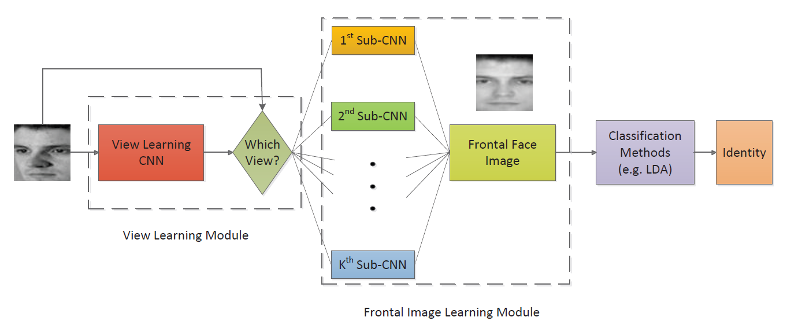
\includegraphics[scale=1]{image3-8}
  \caption{معماری شبکه پیشنهادی \lr{VS2VI}  \cite{7532959}.}
  \label{image3-8}
\end{figure}

\noindent
مدل \lr{VS2VI} از دو بخش اصلی تشکیل شده است. بخش اول به عنوان ورودی یک تصویر خاکستری  شامل یک چهره در هر زاویه و نمای دلخواه با ابعاد 60×60 دریافت می کند و آن را با توجه به نمای چهره طبقه بندی  می کند. سپس تصویر وارد بخش دوم می‌شود که از تعدادی شبکه عصبی پیچشی که هر کدام برای یادگیری تناظر بین یک چهره از رو به رو با یک چهره از یک زاویه و نمای خاص می‌باشد، تشکیل شده است. در این بخش چهره با نمای رو به رو بدست می آید و را مورد شناسایی قرار می دهیم تا هویت فرد مشخص شود. برای این منظور نیز از الگوریتم \lr{LDA} \LTRfootnote{linear discriminant analysis} برای طبقه بندی استفاده شده است. الگوریتم \lr{LDA} برای یادگیری موقعیت چهره استفاده نمی‌شود و فقط برای دسته بندی نهایی مورد استفاده قرار می‌گیرد. معماری این مدل در شکل \ref{image3-9} قابل مشاهده می‌باشد.

\begin{figure}[h]
\centering
  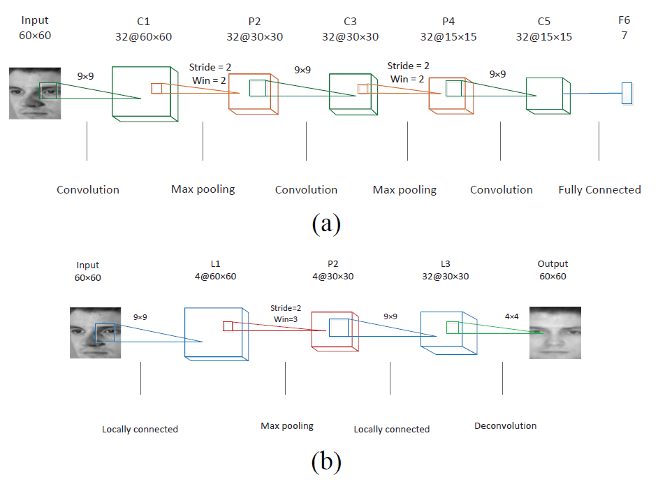
\includegraphics[scale=1]{image3-9}
  \caption{\lr{(a)} معماری مدل یادگیری موقعیت چهره و \lr{(b)} معماری مدل یادگیری بازسازی چهره از رو به رو \cite{7532959}.}
  \label{image3-9}
\end{figure}

\noindent
بخش اول از یک شبکه عصبی پیچشی تشکیل شده است که شامل سه لایه پیچشی، دو لایه رای گیری و یک لایه تمام متصل می‌باشد. ورودی آن یک تصویر با هر موقعیت و زاویه دلخواه و خروجی آن احتمال قرار داشتن تصویر ورودی در هر دسته از دسته های مربوط به نماهای مختلف می‌باشد. برای لایه های پیچشی از تابع فعالیت \lr{ReLU} استفاده شده است. و لایه تمام متصل از \lr{softmax} به عنوان تابع هزینه استفاده کرده است.

\noindent
بخش دوم از تعدادی زیر شبکه پیچشی که هر کدام برای یادگیری تناظر بین چهره از رو به رو با یک چهره از یک نمای خاص می‌باشد، تشکیل شده است. هر یک از این زیر شبکه‌ها شامل دو لایه با اتصال محلی ، یک لایه رای گیری و یک لایه واپیچشی می‌باشند. سه لایه اول برای استخراج ویژگی ها و لایه آخر برای بازیابی چهره از رو به رو می‌باشند. ورودی و خروجی این لایه‌ها تصویر چهره می‌باشد. لایه آخر به جای لایه تمام متصل از لایه واپیچشی استفاده شده است. زیرا حجم محاسبات را به طور قابل توجهی کاهش می‌دهد. یک لایه تماما متصل به 103 میلیون پارامتر نیاز دارد، در حالی که لایه واپیچشی به 460 هزار پارامتر نیاز دارد. لایه اول که اتصال محلی دارد، از تابع \lr{PreLU} به عنوان تابع فعالیت استفاده کرده است. لایه واپیچشی برای نمونه افزایی از درون یابی دو خطی استفاده کرده و تابع هزینه آن $\ell_2-loss$ می‌باشد. برای یادگیری شبکه از الگوریتم پس انتشار خطا \LTRfootnote{Backpropagation} استفاده شده است. الگوریتم \lr{VS2VI} به دقت 95.6\% در تشخیص چهره با زاویه 45 درجه رسیده است.

\noindent
در سال 2018 \lr{Andrey V.Savchenko} و همکاران در \cite{SAVCHENKO2018170} یک روش مبتنی بر \lr{ML} \LTRfootnote{Maximum Likelihood} برای شناسایی چهره در محیط‌های بدون محدودیت با تعداد کم نمونه‌ها بر اساس محاسبه فاصله بین ویژگی‌های با ابعاد بالا که توسط شبکه عصبی پیچشی عمیق مانند \lr{VGG}، \lr{ResNet} و \lr{SENet} استخراج شده است ارائه دادند. این روش جدید شناسایی آماری، احتمال فاصله‌ها را نسبت به تمام تصاویر مجموعه داده‌ها با استفاده از قانون بیز به حداکثر می‌رساند. این احتمال با تخمین توزیع هنجار طبیعی \lr{Kullback–Leibler} بین ویژگی‌های غیرمنفی تخمین زده شده است. این رویکرد بر روی مجموعه داده‌های \lr{LFW}، \lr{YTF} و \lr{IJB-A} مورد آزمایش قرار گرفته است. رویکرد پیشنهادی می‌تواند با استفاده از فواصل سنتی، افزایش دقت 0.3 تا 5.5 درصد در مقایسه با روش‌های شناخته شده داشته باشد، به ویژه اگر تصاویر آموزش و آزمایش تفاوت زیادی داشته باشند. مقایسه روش ارائه شده با سایر روش ها در شکل \ref{image3-10} مشاهده می‌شود.
 
\begin{figure}[h]
\centering
  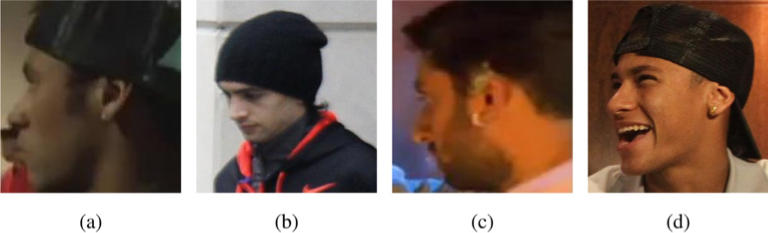
\includegraphics[scale=1]{image3-10}
  \caption{
مقایسه روش ارائه شده با سایر روش ها \lr{(a)} تصویر آزمایشی \lr{(b)} و \lr{(c)} خروجی نادرست روش های دیگر \lr{(d)} خروجی روش ارائه شده \cite{SAVCHENKO2018170}.}
  \label{image3-10}
\end{figure}

\noindent
در سال 2013 \lr{Marsico} و همکاران در \cite{6196234} یک روش رو به رو سازی چهره ارائه دادند. در ابتدا از الگوریتم \lr{STASM} \LTRfootnote{Extended Active Shape Model} برای به دست آوردن 68 نقطه ویژه بر روی چهره استفاده شده است. سپس برای هر تصویر ورودی، شاخص حالت نمونه \lr{(SP)} \LTRfootnote{Simple Pose} محاسبه می‌شود و در صورتی که مقدار آن کمتر از یک آستانه باشد، تصویر مردود شده و در غیر این صورت به مرحله بعد برای هنجارسازی حالت فرستاده می‌شود. هرچه مقدار شاخص \lr{SP} بالاتر باشد، تصویر چهره به حالت تمام رخ نزدیکتر است و اصلاح زاویه کمتری نیاز دارد. شکل \ref{image3-11} قسمت \lr{a} تا \lr{c} معیارهای مورد نیاز برای محاسبه شاخص \lr{SP} را نشان می دهد.

\begin{figure}[h]
\centering
  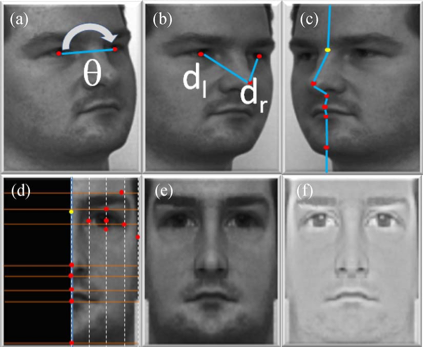
\includegraphics[scale=1]{image3-11}
  \caption{6 مرحله اصلی در فرایند هنجارسازی حالت و روشنایی چهره \cite{6196234}.}
  \label{image3-11}
\end{figure}

\noindent
چرخش: چرخش سر در جهت عقربه‌های ساعت یا عکس آن می‌باشد. و طبق رابطه \ref{eq3-3} به صورت زاویه $\theta$ تعریف می‌شود که زاویه بین خط عبوری از مرکز چشم‌ها و محور افقی $x$ می‌باشد.

\begin{equation}
\label{eq3-3}
roll=min(\left|\frac{2\theta}{\pi}\right|,1)
\end{equation}‏

\noindent	
انحراف: چرخش در راستای محور افقی است و طبق رابطه \ref{eq3-4} مقادیر $𝑑r$ و $𝑑l$ فاصله مرکز چشم چپ و راست از نوک بینی می‌باشد. اندازه گیری این فاصله‌ها در صورت برابر بودن، برای تشخیص تمام رخ بودن تصویر چهره مورد استفاده قرار می‌گیرد.

\begin{equation}
\label{eq3-4}
yaw=\frac{max\left(d_l,d_r\right)-\ min(d_l,d_r)}{max(d_l,d_r)}
\end{equation}‏

\noindent
شیب: برحسب رابطه.\ref{eq3-5} چرخش سر در راستای محور عمودی را اندازه گیری می‌کند.

\begin{equation}
\label{eq3-5}
pitch=\frac{max\left(e_u,e_d\right)-\ min(e_u,e_d)}{max(e_u,e_d)}	
\end{equation}‏

\noindent
با محاسبه 3 شاخص فوق، شاخص \lr{SP} مطابق رابطه \ref{eq3-6} محاسبه می‌شود:

\begin{equation}
\label{eq3-6}
SP=\ \alpha\ .(1-roll)+\ \beta\ .(1-yaw)+\ \gamma\ .(1-pitch)	
\end{equation}

\noindent‏
که در آن‏ 
$\alpha\ +\ \beta\ +\ \gamma=1	$‏
می‌باشد که مقادیر این ضرایب از طریق آزمون و خطا به دست می آیند. سپس در مرحله تمام رخ کردن تصویر چهره، بین دو فاصله \lr{dr} و \lr{dl} هر کدام بزرگتر باشند، نشان می دهد آن سمت از چهره بیشتر در دید دوربین است. اگر نیمه سمت راست صورت به طرف دوربین باشد $(dl \geq dr)$، تصویر بدون تغییر باقی می ماند. در غیر این صورت، تصویر حول محور عمودی برعکس می‌شود که باعث می‌شود همیشه نیمه سمت راست تصویر پردازش شود. سپس برای ثابت کردن طول سطرها، سطرها بسط داده می‌شوند. مطابق شکل \ref{image3-11} قسمت \lr{d} و \lr{e} نیمه سمت چپ تصویر حذف شده و از روی تصویر نیمی از چهره، نیمه دیگر نیز ساخته می‌شود و تصویر تمام رخ چهره به دست می آید.

\section{چالش روشنایی}
متعادل سازی بافت نگار یکی از الگوریتم های مهم در پردازش تصویر است که هدف آن افزایش وضوح تصویر با یکنواخت سازی بافت نگار تصویر است، به گونه ای که بخش های از تصویر که به علت روشنایی کم یا زیاد، پنهان می‌باشند، قابل مشاهده شوند. متعادل سازی بافت نگار قدرتمندترین و رایج ترین روش برای اصلاح روشنایی تصاویر است. اما ضعف این روش، سراسری بودن آن می‌باشد. برای رفع این مشکل باید از الگوریتم‌های محلی استفاده کرد.

\noindent
در سال 2013 \lr{Marsico} و همکاران در \cite{6196234} یک روش هنجار سازی نورپردازی برای تصاویر چهره ارائه دادند و از این روش برای محاسبه شاخص روشنایی نمونه \lr{(SI)} \LTRfootnote{Sample Illumination} استفاده کردند. زمانی که تصویر روشنایی یکنواخت دارد، بیشتر بخش‌های چهره توزیع یکنواخت سطح خاکستری دارند. اما وقتی روشنایی یکنواخت نباشد، برخی از نواحی خاص چهره، توزیع یکنواخت سطح خاکستری ندارند. برای مثال جلوی بینی، گونه‌ها و چانه معمولا نور را منعکس می‌کنند. 8 ناحیه در شکل \ref{image3-12} با توجه به چنین اصلی انتخاب شده اند. 8 بافت نگار با رنگ آبی و مرکز آن ها با رنگ قرمز مشاهده می‌شود.

\begin{figure}[h]
\centering
  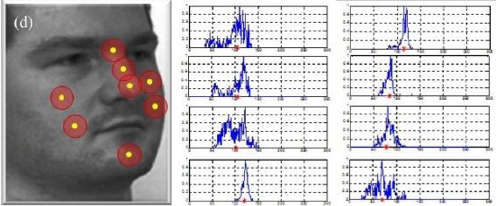
\includegraphics[scale=1]{image3-12}
  \caption{اندازه گیری روشنایی و بافت نگار 8 نقطه خاص \cite{6196234}.}
  \label{image3-12}
\end{figure}

\noindent
8 بافت نگار فوق به یک توزیع یکنواخت با انحراف معیار کم در همسایگی از مرکز حجم بافت نگار اشاره دارد. بافت‌نگار هر یک از ناحیه ها بدست آمده و مرکز ثقل آن مطابق رابطه \ref{eq3-7} محاسبه می‌شود:

\begin{equation}
\label{eq3-7}
mc\left(w\right)=\frac{\sum_{i=0}^{255}{i\times h_w(i)}}{\sum_{i=0}^{255}{h_w(i)}}		
\end{equation}

\noindent
که در آن \lr{w} نشان دهنده یکی از نواحی 8 گانه می‌باشد. 8 مرکز جرم محاسبه شده، بردار \lr{mc} را تشکیل می دهند. با توجه به فرض تشابه ذکر شده در میان نواحی صورت در نظر گرفته شده، انتظار می رود هیچ تنوع قابل توجهی در میان عناصر بردار وجود نداشته باشد و توزیع های یکسانی از سطوح خاکستری را نمایش دهند. برای دستیابی به این منظور پراکندگی مراکز حجم ها از 8 نمودار بافت نگار محاسبه شده است. سپس عناصر بردار \lr{mc} توسط تابع سیگموید \lr{F} در بازه $[1,0]$ هنجارسازی می‌شوند و شاخص کیفیت روشنایی مطابق رابطه \ref{eq3-8} محاسبه می‌شود که یک عدد می‌باشد:

\begin{equation}
\label{eq3-8}
SI=1-F(std\left(mc\right))	
\end{equation}

\noindent
هرچه مقدار \lr{SI} بیشتر باشد، یعنی تصویر روشنایی یکنواخت تری دارد. اگر این شاخص به اندازه کافی رضایت بخش نباشد، تصویر رد می‌شود. در غیر این صورت برای هنجارسازی روشنایی وارد بخش بعدی خواهد شد. در صورت رد شدن تصویر، سیاست های جایگزین برای رسیدگی به این موضوع در دسترس هستند. برای مثال ممکن است یک نمونه جدید درخواست شود که در شرایط برون خط امکان پذیر نیست. یا مداخله انسانی می تواند به صورت دستی نمونه را طبقه-بندی کند. در هر صورت بیشتر بار طبقه بندی بر دوش سامانه خواهد بود. اگر تصویر به مرحله بعد وارد شد، با استفاده از الگوریتم \lr{SQI} توسط یک ماسک مربعی با اندازه 8×8 مقدار هر پیکسل بر مقدار میانگین همسایگانش تقسیم می‌شود و نتیجه نهایی حاصل می‌شود. نتیجه به صورت قسمت \lr{f} در شکل \ref{image3-11} می‌باشد.

\noindent‏
در سال 2015 \lr{Jamal Hussain Shah} و همکاران در \cite{HUSSAINSHAH201597} رویکردی برای تشخیص چهره در تغییرات شدید روشنایی پیشنهاد دادند کرده اند که به سه مرحله تقسیم شده است:
\begin{enumerate}
\item
	برای اصلاح روشنایی غیر یکنواخت، همسان سازی بافت نگار براساس بر اساس ناحیه استفاده می‌شود.
\item 
	ویژگی های مبتنی بر \lr{LDA} از تصویر چهره استخراج می‌شود.
\item
فرایند طبقه بندی بر اساس مدل \lr{OPPM} انجام می‌شود.
\end{enumerate}
	
\section{چالش انسداد}
در سال 2018 \lr{Cho Ying Wu} و همکاران در \cite{WU2018256} یک رویکرد مبتنی بر وايازش  با جهت گرادیان برای شناسایی چهره های در معرض انسداد ارائه دادند. در کاربردهای واقعی، تعداد داده‌های آموزش بسیار کم می‌باشد (شاید یک تصویر به ازای هر شخص). این رویکرد توانایی برخورد با این شرایط را دارد و در مقابل تصاویری که نزدیک به 80 درصد از چهره در شرایط انسداد قرار دارد، به خوبی عمل می‌کند. نتایج نشان می دهد که با تعداد بسیار کمی از تصاویر آموزشی، مدل پیشنهاد شده \lr{GD-HASLR} بهترین عملکرد را در مقایسه با سایر روش های پیشرفته، از جمله روش های مبتنی بر شبکه عصبی پیچشی دارد. مجموعه داده آموزشی $A=\mathbb{R}^{d\times n}$ در نظر گرفته شده که در آن \lr{n} تعداد داده های آموزشی و \lr{d} حاصل ضرب تعداد پیکسل های طول و عرض تصاویر می‌باشد. داده‌های آموزشی چهره های طبیعی و بدون انسداد می‌باشند. $y=\mathbb{R}^d$ یک داده آزمایشی می‌باشد. مطابق رابطه \ref{eq3-9} می‌توان از یک ترکیب خطی داده‌های آموزش برای تخمین زدن داده آزمایش استفاده کرد که شامل یک عبارت خطای $L=\mathbb{R}^d$ نیز می‌باشد.
 
\begin{equation}
\label{eq3-9}
y=Ax+L
\end{equation}

\noindent‏
که در آن \lr{x} بردار ضرایب با \lr{n} بعد می‌باشد. (شکل \ref{image3-13})

\begin{figure}[h]
\centering
  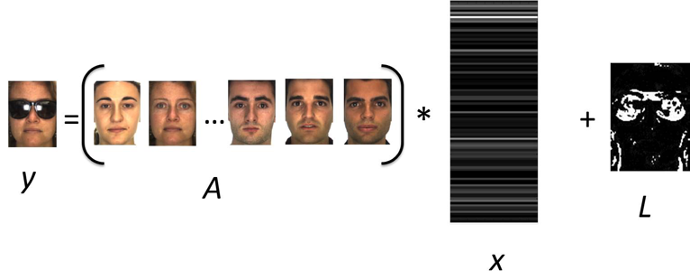
\includegraphics[scale=1]{image3-13}
  \caption{تصویر انسداد از ترکیب خطی تمام چهره های آموزشی در مجموعه داده و یک تصویر \lr{L} که نشان دهنده انسداد است، تشکیل شده است \cite{WU2018256}.}
  \label{image3-13}
\end{figure}

\noindent
برای آنکه شرط تنک بودن به رابطه بالا اضافه شود، مسئله به صورت رابطه \ref{eq3-10} نوشته می‌شود:

\begin{equation}
\label{eq3-10}
arg min ||x||_1   s.t. y - Ax ≤ \epsilon 	
\end{equation}

\noindent‏
که در آن $\epsilon$ یک آستانه خطا می‌باشد. برای تصویر و ورودی و تصاویر مجموعه داده آموزش، گرادیان مرتبه اول، دوم و سوم محاسبه شده و به عنوان ویژگی هر تصویر در نظر گرفته می‌شود. در ادامه شرط کم رتبه بودن ماتریس ویژگی ها نیز به این رابطه اضافه می‌شود. با استفاده از روش ضرایب لاگرانژ، رابطه بالا را می توان به صورت یک مسئله بهینه سازی بدون محدودیت نوشت و حل نمود.

\begin{equation}
\label{eq3-11}
\mathcal{L}(x,L,z) = \alpha ||L_M|| + \sum \pi_\lambda ( |x_i|) + z^T (y - Ax - L) + \frac{\beta}{2} ||y - Ax - L||_2^2
\end{equation}

\noindent‏
که در آن $z$ ضریب لاگرانژ و $\beta$ عامل مجازات می‌باشد. پس از بدست آوردن بردار تنک $x$ می‌توان باقیمانده دسته $i$ ام را به صورت رابطه \ref{eq3-12} محاسبه نمود:

\begin{equation}
\label{eq3-12}
r_i=y-Aδi(x)2
\end{equation}‏

\noindent‏
که در آن $\delta_i(x)$ نشان دهنده $i$ امین انتخاب کننده دسته می‌باشد که فقط ورودی‌های مربوط به دسته $i$ ام را حفظ می‌کند و در سایر قسمت‌ها برابر با صفر می‌باشد. در نهایت دسته ای که کمترین باقیمانده را داشته باشد، انتخاب می‌شود. رویکرد کلی الگوریتم در شکل \ref{image3-14} آمده است.

\begin{figure}[h]
\centering
  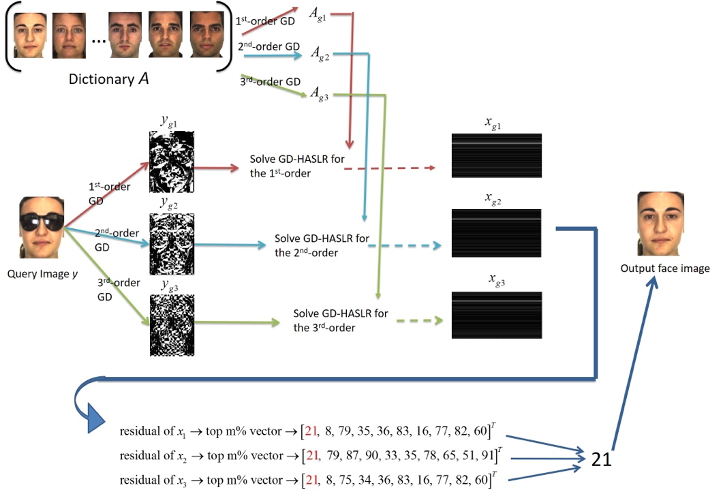
\includegraphics[scale=1]{image3-14}
  \caption{رویکرد کلی الگوریتم \lr{GD-HASLR} \cite{WU2018256}.}
  \label{image3-14}
\end{figure}

\noindent
در سال 2014 \lr{J. Li} و همکاران در \cite{7015448} یک روش تشخیص چهره پوشیده شده در پس زمینه پیچیده ارائه کردند. این الگوریتم از دو مرحله تشکیل شده است. در مرحله اول تعیین می کنند که آیا شی یک شخص می‌باشد یا خیر و در مرحله دوم بررسی می‌شود که آیا چهره پوشیده شده می‌باشد یا خیر و در صورت پوشش چهره، نوع پوشش و اینکه پوشیدگی با ماسک، کلاه، عینک یا ... است را مشخص می کند.

\noindent
در مرحله اول یک رویکرد تشخیص شی در پیش زمینه در حالت پویا و ایستا پیشنهاد شده است. برای تشخیص هدف ایستا از تشخیص مبتنی بر ویژگی \lr{HOG} استفاده شده است. از آنجا که سرعت \lr{HOG} نسبتاً پایین است، از \lr{LBP} به همراه آن نیز استفاده کرده اند. 

\noindent
در مرحله دوم از طبقه بند \lr{Adaboost} برای طبقه بندی چهره های پوشیده شده استفاده شده است که برای انواع پوشیدگی آموزش داده شده است.

\section{چالش کمبود تصاویر آموزشی}
دلیل اصلی به وجود آمدن چالش‌ این است که چهره انسان یک شی صلب نمی‌باشد و ساختار سه بعدی و پیچیده‌ای دارد و ممکن است تصویر از هر زاویه‌ای گرفته شده باشد. بنابراین برای آموزش یک الگوریتم یادگیری که بتواند چهره افراد را از یکدیگر تمیز دهد، نیاز به داده‌های آموزشی بسیاری می‌باشد که در شرایط نورپردازی، زاویه و حالت‌های مختلفی تصویربرداری شده باشد. در مقابل فرض بر این است که داده‌های آموزش بسیار کم هستند. از این رو مسئله تشخیص چهره باید در شرایطی حل شود که داده‌های آموزشی کافی در اختیار نمی‌باشد. بنابراین به الگوریتمی نیاز داریم که به ما کمک کند با تولید داده‌های غیر واقعی، مشکل کمبود داده‌های آموزشی را حل نماییم. از سویی دیگر محدودیت‌ منابع برای اجرای پردازش‌ها بر روی تلفن همراه وجود دارد و الگوریتم ارائه شده باید دارای کمترین پیچیدگی زمانی و حافظه باشد.

\noindent
در سال 2017 \lr{Ya Wang} و همکاران در \cite{7984553} روشی برای تشخیص چهره در دوربین های نظارتی در محیط بدون محدودیت به وسیله شبكه عصبی پیچشی عمیق ارائه دادند. از آنجایی که داده های آموزشی ورودی به مدل از اهمیت بالایی برای تشخیص برخوردار هستند و همچنین به تعداد زیادی از داده های هر دسته برای بهبود عملكرد سامانه نیاز است، نوآوری  این رویکرد، ساختن یک مجموعه داده استاندارد برای شبكه عصبی از روی دوربین های نظارتی در محیط است که در چهار مرحله به صورت زیر ساخته می‌شوند.
\noindent
با توجه به اینكه تصاویر مورد نظر برای هر فرد در مجموعه فریم های پشت سر هم از یک دوربین موجود است، می-توان مجموعه تصاویر یک فرد را بوسیله ترکیب الگوریتم تشخیص چهره و ردیابی چهره جمع آوری کرد. پس از شناسایی یک چهره، با ردیابی آن به وسیله الگوریتم \lr{KCF}، مجموعه تصاویری از آن به عنوان یک دسته طبقه بندی می‌شود.

\begin{figure}[h]
\centering
  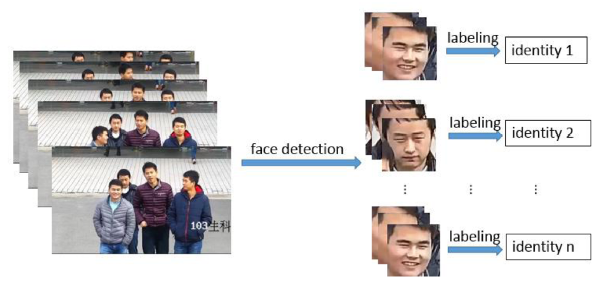
\includegraphics[scale=1]{image3-15}
  \caption{ردیابی، یافتن چهره ها و برچسب زنی \cite{7984553}.}
  \label{image2-1}
\end{figure}

\noindent
	برخی تصاویر در هر دسته به اشتباه در مرحله اول به عنوان تصویر یک فرد در نظر گرفته شده اند (شکل \ref{image3-16}).

\begin{figure}[h]
\centering
  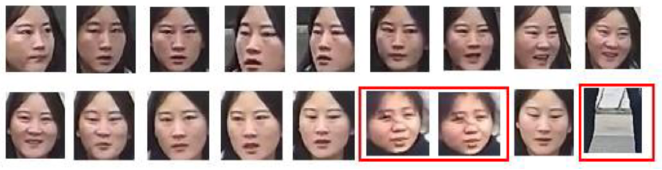
\includegraphics[scale=1]{image3-16}
  \caption{تصاویر با حاشیه قرمز رنگ، به اشتباه برچسب زنی شده اند \cite{7984553}.}
  \label{image3-16}
\end{figure}

\noindent
با استفاده از روش خوشه بندی گراف \LTRfootnote{Graph Clustering} روی ویژگی های استخراج شده از شبكه \lr{VGG-Face}، تشخیص و پاک سازی تصاویر اشتباه انجام می‌شود. فاصله کسینوسی بین ویژگی های تصاویر چهره محاسبه می‌شود و اگر این فاصله برای هر دو تصویر کمتر از یک مقدار آستانه باشد، این تصاویر متعلق به یک فرد هستند. با توجه به شکل \ref{image3-17} تصویری که بیشترین شباهت را به تصاویر دیگر دارد، به عنوان شاخص برای آن شخص انتخاب می‌شود.

\begin{figure}[h]
\centering
  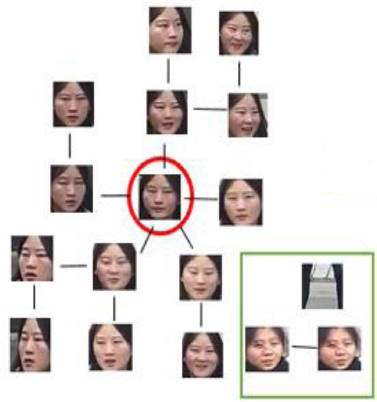
\includegraphics[scale=1]{image3-17}
  \caption{ استفاده از روش خوشه بندی گراف و تعیین تصویر شاخص \cite{7984553}.}
  \label{image3-17}
\end{figure}

\noindent
	با استفاده از محاسبه فاصله بین هر داده با داده مرکزی و در نظر گرفتن یک آستانه، داده های تكراری در هر دسته مشخص شده و حذف می‌شوند. با توجه به مقدار داده‌های درون هر دسته، تصفیه بین دسته ای انجام می‌شود. اگر مجموعه داده های درون هر دسته کمتر از 100 تصویر باشد، آن دسته از مجموعه داده حذف می‌شود. دقت خوشه بندی و جمع آوری مجموعه داده 99.2\% شده است. در نهایت از یک مدل پیش آموزش دیده شده شبكه \lr{VGG-Face} همراه با \lr{Fine-tuning} برای طبقه بندی تصاویر آزمایشی استفاده شده است که به دقت 92.1\% رسیده است.

\noindent
مقاله \cite{radford2016unsupervised} از شبکه‌های مولد تخاصمی‌برای تولید داده‌ها استفاده کرده است که به اختصار \lr{GAN} نامیده می‌شوند. \lr{GAN} از دو شبکه مستقل تولید کننده و تمیز دهنده استفاده تشکیل شده است. شبکه تولید کننده از روی بردار $Z$ که می‌تواند یک نویز تصادفی باشد، یک تصویر تولید می‌کند و شبکه تمیز دهنده وظیفه دارد تصاویر واقعی را از تصاویر تولید شده توسط شبکه تولید کننده تشخیص دهد. بنابراین هر تصویر با یک بردار $Z$ معرفی می‌شود. در این مقاله محاسبات در فضای برداری انجام شده و بردار حاصل، تبدیل به تصویر خروجی می‌شود. به عنوان مثال بردار $Z$ برای تصویر خانمی که عینک آفتابی نزده است از بردار $Z$ برای تصویر خانمی که عینک آفتابی زده است، کم می‌شود و حاصل آن، بردار مربوط به یک عینک آفتابی می‌باشد. سپس این بردار با بردار تصویر آقایی که عینک نزده است جمع می‌شود. نتیجه نهایی تصویر همان آقا با عینک آفتابی می‌باشد. به عنوان مثالی دیگر، با میانگین گیری بردارهای مربوط به دو تصویر از چهره شخصی که به سمت راست و چپ متمایل است، توانسته چهره رو به روی شخص را بازسازی نماید. اما کیفیت کار هنوز تا حالت مطلوب فاصله دارد. نمونه ای از خروجی این روش در شکل \ref{image3-18} قابل مشاهده می‌باشد.

\begin{figure}[h]
\centering
  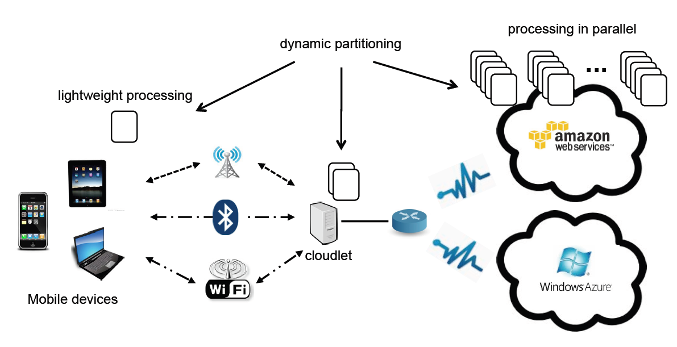
\includegraphics[width=1.0\textwidth]{image3-18}
  \caption{تولید تصاویر چهره از زوایای مختلف با استفاده از درونیابی بردارهای تصاویر چپ و راست \cite{radford2016unsupervised}.}
  \label{image3-18}
\end{figure}

\noindent
مقاله \cite{BANERJEE2018246} یک شبکه عمیق مبتنی بر \lr{GAN} را با نام \lr{LR-GAN} پیشنهاد می‌دهد، که تصاویر واقع گرایانه با وضوح بالا را از روی تصاویر با وضوح پایین بازسازی می‌کند. این تصاویر چهره غیر واقعی اما واقع گرایانه و با کیفیت، باعث عملکرد بهتر سامانه شناسایی چهره برای مقایسه تصاویر می‌شود. رویکرد اصلی مقاله در روش آموزش تخاصمی \lr{LR-GAN} بهینه سازی تابع ضرر بازسازی چند مقیاسی  است، بر اساس شاخص‌های مانند: شاخص شباهت ساختاری چند مقیاسی \lr{(SSIM)}، میانگین مربعات خطا برای هر قسمت  \lr{(PMSE)}، واگرایی جنسن شانون اصلاح شده  \lr{(JSD)} و تنوع متقابل در اطلاعات \lr{(MVI)}.  شبکه تمیز دهنده در \lr{LR-GAN}، بر اساس اطلاعات طبقه‌ بندی که به طور ضمنی در طول آموزش آموخته می‌شود، هویت هر شخص را حفظ می‌کند. این رویکرد سریعتر از شبکه‌های مبتنی بر \lr{GAN} اخیر به یک همگرایی می‌رسد. این مدل که به دقت بالای90\% رسیده است، رتبه اول را در 4 مجموعه داده شرایط بدون محدودیت کسب کرده است. نمونه ای از خروجی این روش در شکل \ref{image3-19} قابل مشاهده می‌باشد.

\begin{figure}[h]
\centering
  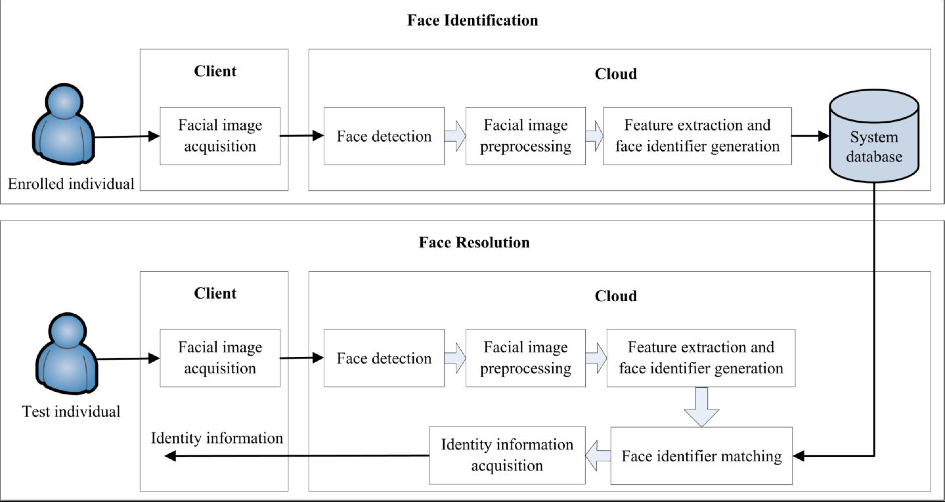
\includegraphics[width=1.0\textwidth]{image3-19}
  \caption{
تولید تصویر با وضوح بالا از روی تصاویر با وضوح پایین در 4 مجموعه داده مختلف. موارد با حاشیه قرمز خروجی اشتباه هستند
  \cite{BANERJEE2018246}.}
  \label{image3-19}
\end{figure}

\noindent
شبکه‌های \lr{GAN} یاد می‌گیرند تصاویر جدیدی تولید کنند که شبیه به تصاویر واقعی باشند. اما این شبکه‌ها معمولا کنترل کمی روی ویژگی‌های بصری تصاویر خروجی دارند. مقاله \cite{karras2019stylebased} یک شبکه \lr{GAN} جدید پیشنهاد می‌دهد که بخش تولید کننده آن به طور خودکار یاد می‌گیرد بدون هیچ ناظر انسانی ویژگی‌های بصری متفاوت تصاویر را از یکدیگر جدا نماید. پس از اتمام مرحله یادگیری، ما می‌توانیم این ویژگی‌های بصری را به دلخواه خود ترکیب نماییم. برای مثال ویژگی‌های اساسی مانند جنسیت، سن، طول مو، وجود عینک و زاویه چهره را از تصویر 1 با ویژگی‌های دیگری از تصویر 2 ترکیب کرد و یک چهره جدید تولید نمود. نگاه این شبکه تولید کننده به هر تصویر، مجموعه ای از ویژگی‌های بصری می‌باشد. هر ویژگی بصری با اندازه مشخص، جلوه‌های تصویر را کنترل می‌کند. ویژگی‌های بصری غالب مانند زاویه چهره، مو، شکل صورت؛ ویژگی‌های بصری میانی مانند فرم لب و چشم‌ها و ویژگی‌های سبک تر مانند رنگ. ما می‌توانیم این ویژگی‌های بصری را با ضرایب دلخواه خود ترکیب نماییم. نمونه ای از خروجی این روش در شکل \ref{image3-20} قابل مشاهده می‌باشد.
 
\begin{figure}[h]
\centering
  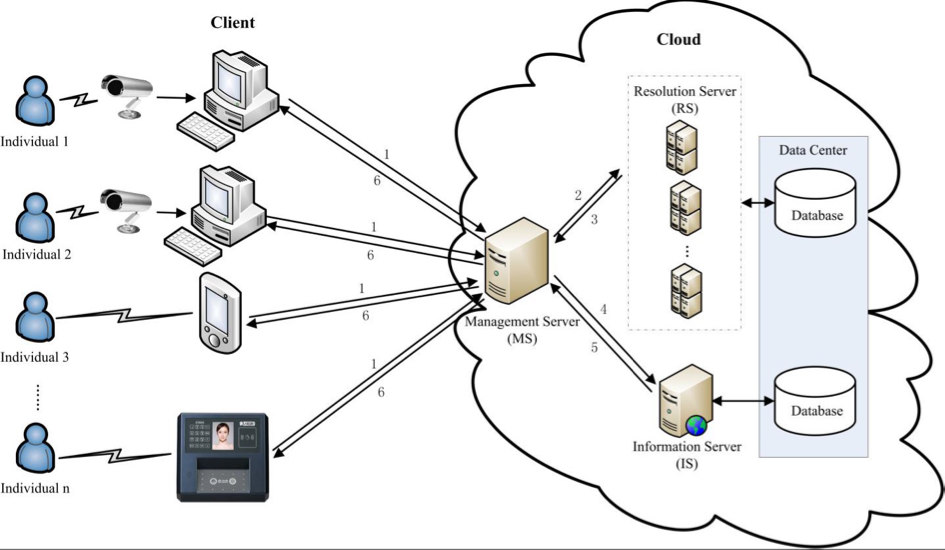
\includegraphics[width=1.0\textwidth]{image3-20}
  \caption{
تصاویر هر ردیف و هر ستون دارای برخی ویژگی‌های دیداری مشابه هستند 
  \cite{karras2019stylebased}.}
  \label{image3-20}
\end{figure}

\noindent
در مقاله \cite{8603840} به موضوع تولید چهره در زوایای دلخواه پرداخته شده است. در این مقاله از دو شبکه \lr{GAN} استفاده شده است که در شبکه اول از روی چهره زاویه‌دار، چهره روبه‌رو تولید شده است. سپس با استفاده از شبکه \lr{GAN} دوم از روی تصویر چهره روبه‌رو، تصویر با زاویه دلخواه با استفاده از یک پارامتر کنترلی تولید می‌شود. چالشی که در این مقاله به آن اشاره شده است، مسئله عدم توازن داده‌ها در وجود برخی ویژگی‌ها در تصاویر می‌باشد. این مقاله در برخی تصاویر چهره زاویه‌دار به مشکل برخورد می‌کرد. به عنوان مثال چهره‌هایی که دارای عارضه‌های پوستی می‌باشند توسط شبکه‌ها نادیده گرفته شده و تصویر چهره روبه‌رو بدون عارضه تولید شده است. این چالش از جایی نشات می‌گیرد که تصاویر با عارضه پوستی در مجموعه داده بسیار کم می‌باشند و شبکه در مواجه با این مسئله ایده‌ای برای آن ندارد و فقط جهت چهره را تغییر می‌دهد و بافت غالب صورت را بر روی صورت خروجی اعمال می‌کند. نمونه ای از خروجی این روش در شکل \ref{image3-20} قابل مشاهده می‌باشد.

\begin{figure}[h]
\centering
  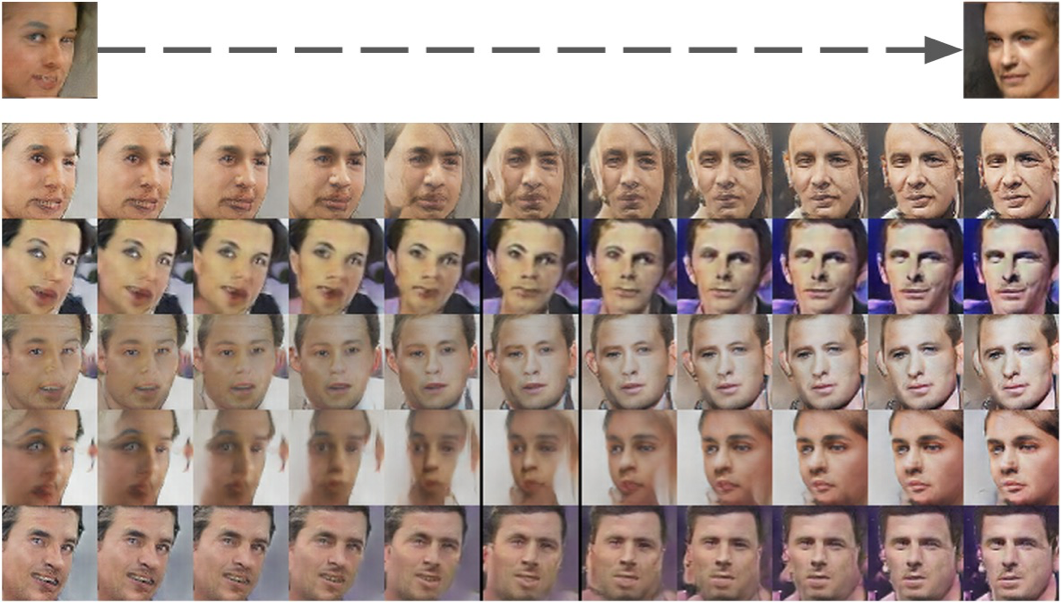
\includegraphics[width=1.0\textwidth]{image3-21}
  \caption{ساختار شبکه \lr{AD GAN} - شبکه \lr{GN} برای رو به رو سازی چهره و شبکه \lr{GE} برای تولید چهره از زوایای مختلف \cite{8603840}.}
  \label{image3-21}
\end{figure}
 
\section{چالش منابع محدود}
در سال 2012 \lr{Tolga Soyata} و همکاران در \cite{6249269} یک روش تشخیص چهره بی درنگ مبتنی بر بینایی ابری \LTRfootnote{Cloud Vision} با استفاده از معماری \lr{MOCHA} ارائه کردند (شکل \ref{image3-22}). با فراگیر شدن تلفن همراه هوشمند در میان شهروندان، سامانه تشخیص چهره می تواند از همکاری مشترک محاسبات تلفن همراه و رایانش ابری استفاده کند. چالش این سامانه، چگونگی تجزیه انجام وظیفه بین تلفن همراه و فضای ابری، توزیع بار محاسبه در میان سرورهای ابر برای به حداقل رساندن زمان پاسخ با توجه به تأخیر ارتباطات مختلف و قدرت محاسبه سرور می‌باشد. نتایج نشان می دهد که الگوریتم-های بخش بندی بهینه پردازش بین تلفن همراه و فضای ابری با توجه به زمان تأخیر ناهمگن، توانایی محاسبه را به طور قابل توجهی افزایش می دهند. 

\begin{figure}[h]
\centering
  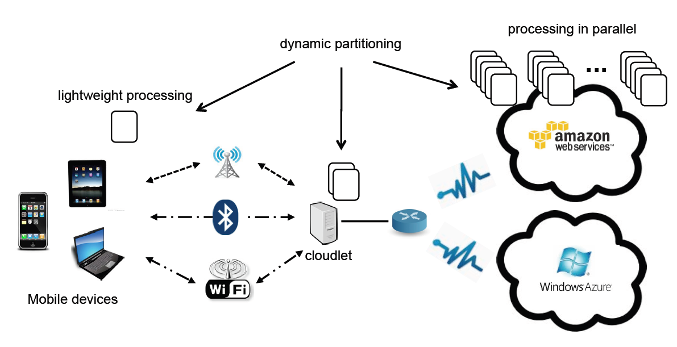
\includegraphics[width=1.0\textwidth]{image3-22}
  \caption{معماری \lr{MOCHA}: دستگاه های تلفن همراه از طریق اتصال چندگانه با \lr{cloudlet} و ابر ارتباط برقرار می‌کنند \cite{6249269}.}
  \label{image3-22}
\end{figure}

\noindent
این سامانه از لحاظ ساختار به سه بخش تقسیم می‌شود:

\noindent
دستگاه همراه: تلفن های همراه و \lr{iPad} ها نقش تهیه و ارسال تصاویر را دارند. تصاویر با فرمت \lr{RAW} فرستاده می‌شوند تا قابلیت پیش پردازش بهتری داشته باشند. اگر سرور ابر به دستگاه همراه نزدیک باشد و ارتباط با سرعت بالا امکان پذیر باشد، تصاویر پیش پردازش به سرور فرستاده می‌شوند. در غیر این صورت مرحله پیش پردازش در دستگاه همراه انجام می‌شود و فقط اطلاعاتی همچون ویژگی های \lr{Haar} و طبقه بندها به سرور فرستاده می‌شوند. پس از اتمام فرایند تشخیص چهره، نتیجه نهایی برای تلفن همراه فرستاده می‌شود.

\noindent
ابر کوچک : سرورها و رایانه هایی که توانایی پردازشی متوسطی دارند، ابر کوچک یا \lr{cloudlet} نامیده می‌شوند. این دستگاه ها که به عنوان میان دستگاه های همراه و سرورهای ابری اصلی قرار دارند، مجهز به \lr{GPU} می‌باشند تا بتوانند پردازش موازی را در زمان مطلوبی انجام دهند.

\noindent
ابر: سرورهای ابر دارای توان پردازشی و پاسخگویی بسیار بالا می‌باشند که بار محاسبات سنگین سامانه را به دوش می کشند و تصمیم گیری نهایی بر روی آن انجام می پذیرد.

\noindent
در سال 2018 \lr{Pengfei Hu} و همکاران در \cite{HU2018582} یک رویکرد تشخیص چهره مبتنی بر رایانش ابری ارائه کردند. افزایش برنامه های کاربردی در زمینه کلان داده ها\LTRfootnote{Big Data} باعث افزایش تقاضای سامانه های شناسایی چهره برای محاسبات قدرتمند و ظرفیت ذخیره سازی بالا می‌شود. این سامانه به طور کامل از مزایای محاسبات ابری بهره می‌برد تا به طور موثر توانایی محاسبات و ظرفیت ذخیره سازی را بهبود بخشد. نتایج تجربی نشان می دهد که طرح پیشنهادی عملا امکان-پذیر است و می تواند سرویس شناسایی موثر چهره را فراهم کند. همانطور که در شکل \ref{image3-23} مشاهده می‌شود، تنها تهیه تصویر بر عهده دستگاه سرویس گیرنده می‌باشد و تمام محاسبات یافتن و شناسایی چهره بر روی ابر انجام می‌شود.
 \begin{figure}[h]
\centering
  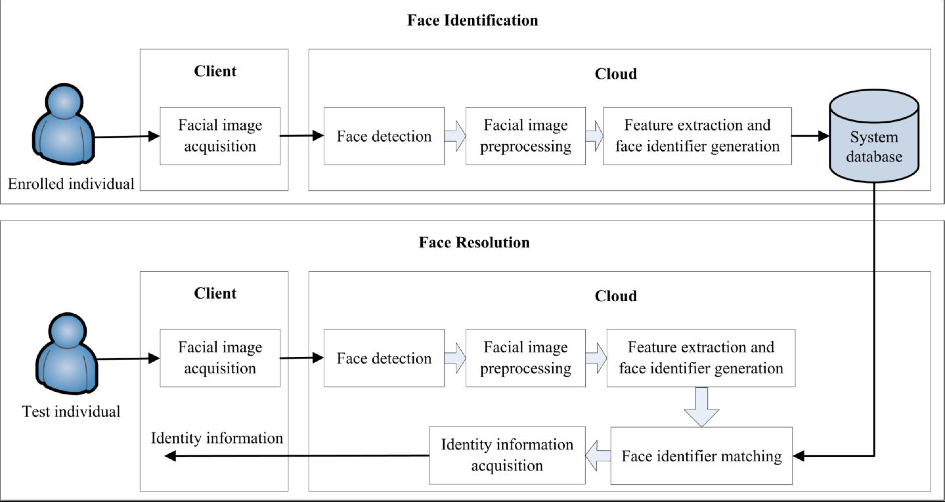
\includegraphics[width=1.0\textwidth]{image3-23}
  \caption{نمای کلی سامانه تشخیص چهره مبتنی بر رایانش ابری \cite{HU2018582}.}
  \label{image3-23}
\end{figure}

\noindent
در این سامانه تصویر با فرمت RAW برای ابر ارسال شده و برای یافتن چهره از ویژگی های Haar استفاده شده است. سپس عملیات همسان سازی بافت نگار بر روی تصویر چهره اعمال می‌شود تا بهبود جزیی حاصل شود. سپس از الگوریتم LBP \LTRfootnote{Local Binary Patterns}برای استخراج ویژگی های چهره استفاده شده، برای هر تصویر یک شناسه تولید می گردد و در نهایت با استفاده از فاصله اقلیدسی با شناسه تصاویر موجود در پایگاه داده مطابقت داده می‌شود. همانطور که در شکل \ref{image3-24} مشاهده می‌شود این سامانه ابری از بخش های سرور مدیریت (MS)\LTRfootnote{Management Server}، سرور اطلاعات (IS)\LTRfootnote{Information Server}، سرور شناسایی (RS)\LTRfootnote{Resolution Server} و پایگاه داده تشکیل شده است. به علت قدرت بالای پردازش در سرور ابری، امکان پردازش موازی نیز در این سامانه وجود دارد که باعث افزایش سرعت محاسبات و کاهش زمان پاسخ دهی سامانه می گردد. 

\begin{figure}[h]
\centering
  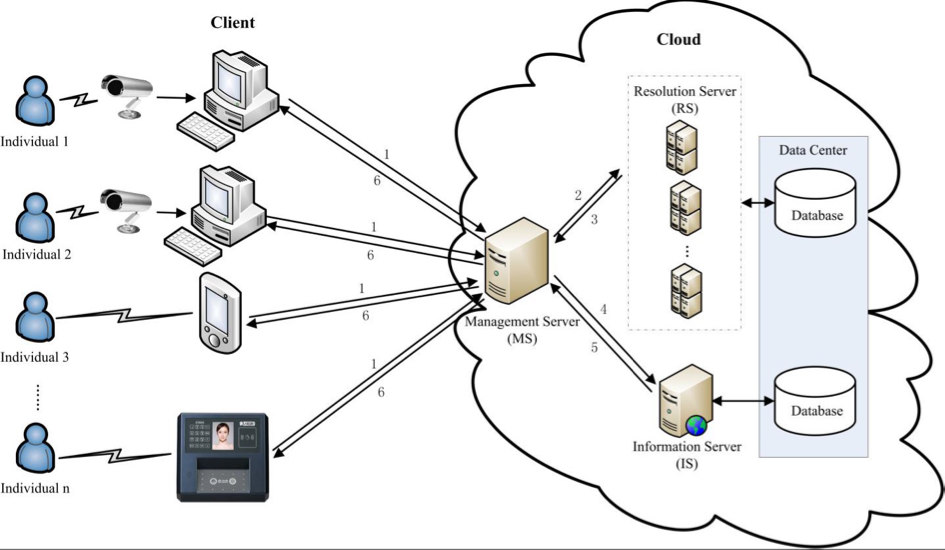
\includegraphics[width=1.0\textwidth]{image3-24}
  \caption{چارچوب سامانه شناسایی چهره مبتنی بر رایانش ابری \cite{HU2018582}.}
  \label{image3-24}
\end{figure}

\noindent
علاوه بر رویکردهای بالا که هر یک بر روی حل یک مسئله خاص تمرکز کرده بودند، برخی روش‌هایی که اخیرا معرفی شده اند، سعی بر این داشته اند که یک راه حل نسبتا همه جانبه در مورد مسئله تشخیص چهره و مشکلات آن ارائه دهند. یکی از این رویکردها، استفاده از تابع ضرر CosFace می‌باشد که در سال ۲۰۱۸ \lr{Wang} و همکاران در \cite{wang2018cosface} ارائه دادند. این تابع ضرر کسینوسی با حاشیه زیاد \LTRfootnote{Large Margin Cosine Loss} شباهت بسیار زیادی به تابع ضرر \lr{softmax} دارد. با این تفاوت که به جای ضرب ماتریس ضرب های \lr{W} در بردار ویژگی \lr{x}، حاصل ضرب مقادیر موجود در ویژگی های استخراج شده و آخرین لایه کامل
متصل را به صورت
$W_j^T x_i = ||W_j|| ||x_i|| cos(θ_j)$
تبدیل می کند، که $\theta_j$ زاویه بین وزن $W_j$ و ویژگی $x_i$ است.

\begin{equation}
\label{eq3-13}
L = - \frac{1}{N} \sum_{i=1}^{N} log \frac{e^{s(cos(\theta_{y_i}-m))}}{e^{s(cos(\theta_{y_i}-m))} + \sum_{j=1}^{n} e^{s(cos(\theta_{j, i}))}}
\end{equation}

\noindent
همانطور که در شکل \ref{image3-25} نشان داده شده است، \lr{softmax} ویژگی‌های تقریباً قابل تفکیکی ایجاد می‌کند اما در مرزهای تصمیم گیری ابهام قابل توجهی به وجود می‌آید، در حالی که تابع ضرر معرفی شده می‌تواند فاصله بیشتری را بین دسته‌های نزدیک اعمال کند.

\begin{figure}[h]
\centering
  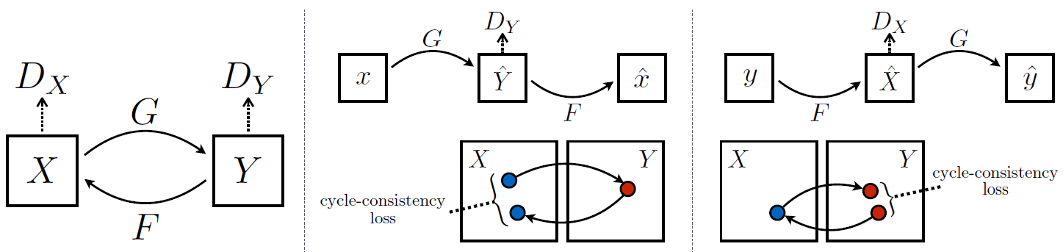
\includegraphics[width=0.5\textwidth]{image3-25}
  \caption{تابع ضرر \lr{CosFace} حاشیه بیشتری نسبت به \lr{SoftMax} در مرز بین دسته ها ایجاد می‌نماید \cite{wang2018cosface}.}
  \label{image3-25}
\end{figure}

\noindent
در سال ۲۰۱۹ Deng و همکاران در \cite{deng2019arcface} یک تابع ضرر پیشنهاد دادند که کمک می‌کند ویژگی‌های استخراج شده که متعلق به دو دسته متفاوت هستند، فاصله بیشتری از هم داشته باشند و در مقابل ویژگی های استخراج شده برای دو تصویر از چهره یک فرد یکسان، فاصله کمتری از هم داشته باشند؛ این روش که به دنبال مقاله \cite{wang2018cosface} آمده است. سعی در بهبود روش پیشین و افزایش دقت کرده است. برای آموزش شبکه های عصبی عمیق پیوسته برای تشخیص چهره، دو رویکرد اصلی وجود دارد. روش اول دسته بندی را آموزش می دهند که می تواند هویت های مختلف را در مجموعه آموزش از هم جدا کند، مانند استفاده از طبقه بندی \lr{softmax}، و رویکرد دوم که مستقیماً یک تعبیه را یاد می گیرند، مانند \lr{triplet loss}. بر اساس داده های آموزش در مقیاس بزرگ و معماری \lr{DCNN}، هر دو روش می توانند عملکرد بسیار خوبی در تشخیص چهره داشته باشند. با این حال، هم رویکرد \lr{softmax} و هم رویکرد \lr{triplet loss} اشکالاتی دارد.
\noindent
برای \lr{softmax}:
\begin{enumerate}
\item
	اندازه ماتریس تبدیل W به طور خطی با افزایش تعداد دسته ها \lr{(n)} افزایش می یابد.‌
\item 
ویژگیهای آموخته شده برای مسئله‌های طبقه بندی با مجموعه بسته قابل تفکیک هستند اما به اندازه کافی برای مسئله تشخیص چهره که یک مسئله باز می‌باشد، مناسب نیستند. 
\end{enumerate}

\noindent
برای \lr{triplet loss}:
\begin{enumerate}
\item
 برای مجموعه داده های مقیاس بزرگ، رشد شدید در تعداد ترکیب‌های تعداد تصاویر سه گانه وجود دارد که منجر به افزایش قابل توجه تعداد مراحل تکرار می‌شود.
\item 
 استخراج مجموعه تصاویر سه گانه یک مسئله دشوار برای آموزش موثر می‌باشد. 
\end{enumerate}

\noindent
برای افزایش بیشتر قدرت تمایز مدل تشخیص چهره و ایجاد ثبات در روند آموزش، تابع ضرر مبتنی بر توابع مثلثاتی پیشنهاد شده است. حاصل ضرب نقطه ای مقادیر موجود در ویژگی های استخراج شده و آخرین لایه کاملاً متصل، برابر با ضرب کسینوسی آن‌ها پس از نرمال سازی می‌باشد‌. از تابع مثلثاتی کسینوسی برای محاسبه زاویه بین ویژگی فعلی و وزن هدف استفاده شده ‌است. سپس یک حاشیه زاویه ای به زاویه هدف اضافه شده‌، در انتها دوباره مقادیر به فضای خطی برگردانده شده است. مراحل بعدی دقیقاً مانند \lr{softmax} هستند. مزایای این روش پیشنهادی را می‌توان به شرح زیر خلاصه کرد:
\begin{itemize}
 \item
در مجموعه داده های تصویر و فیلم در مقیاس بزرگ ، به عملکرد مناسبی دست می یابد.
 \item
فقط به چندین خط کد نیاز دارد و اجرای آن در چارچوب های یادگیری عمیق مبتنی بر \lr{Pytorch} و \lr{Tensorflow} آسان است. برای داشتن عملکرد پایدار نیازی به ترکیب با سایر توابع ضرر ندارد و به راحتی همگرا می‌شود.
 \item
هنگام آموزش فقط پیچیدگی محاسباتی ناچیز را اضافه می کند. پردازنده های گرافیکی کنونی می توانند به راحتی از هزاران دسته مختلف برای آموزش پشتیبانی کنند و مدل به راحتی می تواند هویت های بیشتری را پشتیبانی کند.
\end{itemize}
 
\noindent
رابطه ریاضی \lr{softmax} معروف ترین تابع ضرر طبقه بندی که به طور گسترده استفاده می‌شود، به شرح زیر است:

\begin{equation}\label{eq3-14}
L= - \frac{1}{N} \sum_{i=1}^{N} log \frac{e^{{W_{y_i}^T} x_i + b_{y_i}}}{\sum_{j=1}^{n} e^{{W_j^T} x_i + b_j}} 
\end{equation}

\noindent
که در آن \lr{xi} نشان دهنده ویژگی عمیق نمونه \lr{i} ازدسته \lr{y} است. تعداد ابعاد ویژگی استخراج شده را 512 در نظر گرفتیم. \lr{Wj} ستون \lr{j}  ام از وزن \lr{W} می‌باشد و \lr{bj} بایاس است. مقدار \lr{N}اندازه دسته و \lr{n} تعداد دسته‌ها است. این تابع مستقیما ویژگی استخراج شده را برای اعمال شباهت بالاتر برای نمونه های درون کلاس و فاصله بیشتر برای نمونه های بین کلاسی بهینه نمی‌کند، که منجر به ایجاد مشکل در عملکرد آن برای تشخیص چهره عمیق تحت تغییرات ظاهری بزرگ درون کلاس می‌شود (به عنوان مثال تغییرات زاویه چهره و تقییرات سنی).

\noindent
ما رابطه فوق را مبنای محاسبات قرار دادیم و تغییرات جزیی به آن اضافه کردیم. برای سادگی مقدار بایاس را صفر در نظر گرفتیم. سپس حاصل ضرب مقادیر موجود در ویژگی های استخراج شده و آخرین لایه کامل متصل را به صورت
$W_j^T x_i = ||W_j|| ||x_i|| cos(θ_j)$
تبدیل می کنیم، که \lr{θj} زاویه بین وزن \lr{Wj} و ویژگی \lr{xi} است. نرمال سازی ویژگی‌ها و وزن‌ها باعث می‌شود که خروجی فقط به زاویه بین ویژگی و وزن بستگی داشته باشد. به کمک نرمال سازی مقادیر وزن $||W_j||$ را برابر ۱ در نظر می‌گیریم. همچنین ویژگی استخراج شده $||x_i||$ را نرمال کرده و نام آن را \lr{s} در نظر می‌گیریم. ‌‌‌بنابرین ویژگی‌های استخراج شده در یک ابر کره با شعاع s توزیع می‌شوند. برای افزایش حاشیه بین \lr{xi} و \lr{Wj} یک مقدار \lr{m}اضافه می‌کنیم تا به طور همزمان فشرده سازی درون کلاسی و اختلاف بین کلاسی را افزایش دهیم.

\begin{equation}\label{eq3-15}
L = - \frac{1}{N} \sum_{i=1}^{N} log \frac{e^{s(cos(\theta_{y_i}+m))}}{e^{s(cos(\theta_{y_i}+m))} + \sum_{j=1, j\neq y_i}^{n} e^{s(cos(\theta_j))}}
\end{equation}

\noindent
همانطور که در شکل \ref{image3-26} نشان داده شده است، \lr{softmax} ویژگی‌های تقریباً قابل تفکیکی ایجاد می‌کند اما در مرزهای تصمیم گیری ابهام قابل توجهی به وجود می‌آید، در حالی که تابع ضرر ما می تواند فاصله بیشتری را بین دسته‌های نزدیک اعمال کند.

\begin{figure}[h]
\centering
  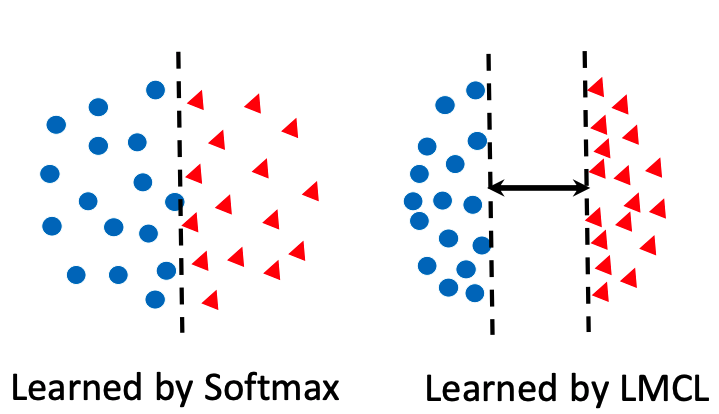
\includegraphics[width=0.5\textwidth]{image3-26}
  \caption{رویکردهای مختلف هم ترازی چهره \cite{deng2019arcface}.}
  \label{image3-26}
\end{figure}

\noindent
این روش دقت 99.53 را بر روی مجموعه داده LFW با معماری ResNet50 بدست آورده است. خلاصه این روش در شکل \ref{image3-27} آمده است.

\begin{figure}[h]
\centering
  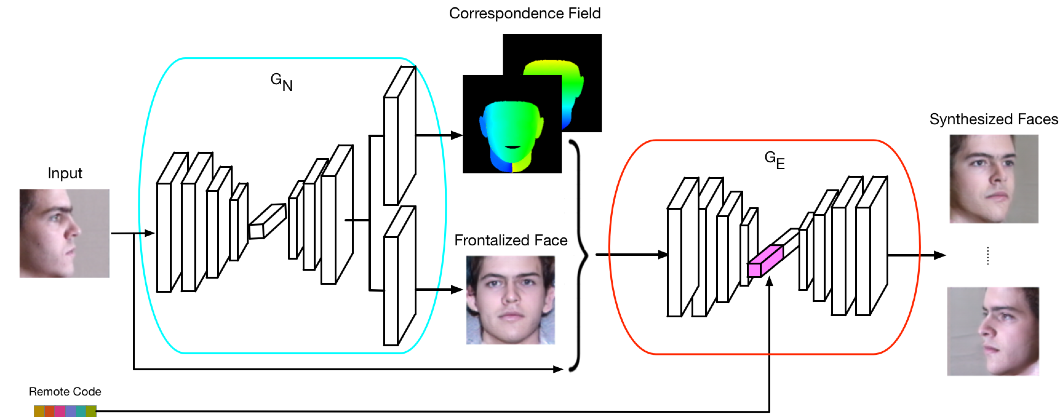
\includegraphics[width=1.0\textwidth]{image3-27}
  \caption{رویکردهای مختلف هم ترازی چهره \cite{deng2019arcface}.}
  \label{image3-27}
\end{figure}

\section{نتیجه گیری}
بیشتر سامانه‌های تشخیص چهره عملکردهای قابل قبولی را در محیط‌های کنترل شده ارائه می‌دهند، اما در محیط‌های بدون محدودیت و در معرض تخریب شدید تصاویر چهره، عملکرد خوبی ندارند و در کاربردهای واقعی هنوز مسیری طولانی برای بهبود در پیش دارند. از جمله چالش‌های مهم، اساسی و عمومی در سامانه‌های تشخیص چهره می‌توان به موارد زیر اشاره نمود:

\begin{itemize}
\item
تشخیص چهره در محیطی با تغییرات شدید نورپردازی مانند روز و شب \lr{(illumination)}
 \item
تغییر زاویه و حالت چهره نسبت به دوربین \lr{(pose)}
 \item
انسداد صورت توسط اشیایی مانند عینک آفتابی و شال گردن \lr{(occlusion)}
 \item
تغییرات اساسی در چهره با گذر زمان، مانند رشد موها و ریش‌ها و یا بالا رفتن سن مانند سفید شدن موها \lr{(aging)}
 \item
تاری خارج از تمرکز دوربین \lr{(bluring)}
 \item
وضوح پایین تصویر \lr{(low resolution)}
 \item
ردیابی چهره در فریم‌های ویدیو با در نظر گرفتن تناظر بین فریمی \lr{(face tracking)}
\end{itemize}

\noindent
دلیل اصلی به وجود آمدن چالش‌ها این است که چهره انسان یک شی صلب نمی‌باشد و ساختار سه بعدی و پیچیده‌ای دارد و ممکن است تصویر از هر زاویه‌ای گرفته شده باشد. بنابراین برای آموزش یک الگوریتم یادگیری که بتواند چهره افراد را از یکدیگر تمیز دهد، نیاز به داده‌های آموزشی بسیاری می‌باشد که در شرایط نورپردازی، زاویه و حالت‌های مختلفی تصویربرداری شده باشد.

\noindent
مقاله \cite{HAGHIGHAT201623} روشی برای رو به رو سازی تصویر چهره پیشنهاد کرده بود که در برخی موارد، چهره را به خوبی میچرخاند، اما در نیمی از مواقع نیز نتیجه خروجی الگوریتم، تصویر چهره را دچار اعوجاج‌هایی می‌نماید که روند تشخیص چهره را با مشکل بیشتری مواجه می‌سازد. از این رو فرایند رو به رو سازی به طور میانگین کمک شایانی به بالا رفتن دقت تشخیص چهره نمی‌نماید.

\noindent
مقاله \cite{radford2016unsupervised} روشی مبتنی بر \lr{GAN} برای تغییر زاویه چهره پیشنهاد داده بود که این الگوریتم نیز در برخی مواقع به تصویر چهره لطمه وارد می‌نماید به طوری که شخص مورد نظر قابل شناسایی توسط سامانه یادگیری نمی‌باشد.

\noindent
مقاله  \cite{BANERJEE2018246} در تولید تصاویر با وضوح بالا بسیار موفق عمل کرده است. اما سایر موارد چالش برانگیز را مورد توجه قرار نداده است. برای مثال اصلاح نورپردازی و زاویه چهره را نادیده گرفته است.

\noindent
در مقاله \cite{8603840} چهره‌هایی که دارای عارضه‌های پوستی می‌باشند توسط شبکه‌ها نادیده گرفته شده و تصویر چهره روبه‌رو بدون عارضه تولید شده است. این چالش به خاطر کمبود تصاویر با عارضه پوستی در مجموعه داده می‌باشد و شبکه در مواجه با این مسئله راه‌کاری ارائه نمی‌دهد و فقط جهت چهره را تغییر می‌دهد و بافت غالب صورت را بر روی صورت خروجی اعمال می‌کند.
\noindent
به تازگی یادگیری عمیق در تشخیص چهره و بسیاری از زمینه های هوش مصنوعی به راه حل غالب تبدیل شده است. ما یک سوال مطرح می کنیم: آیا یادگیری عمیق واقعا مسئله تشخیص چهره را حل می کند؟ چالش روش های یادگیری عمیق در تشخیص چهره چیست؟ 
\noindent
در مقایسه با تشخیص شیء عمومی، تشخیص چهره به دلیل طیف گسترده ای از تغییرات در ظاهر چهره ها چالش برانگیز است. نورپردازی کنترل نشده، انسداد ناشی از عینک، مو، ریش، کلاه و... ، تاری خارج از تمرکز دوربین، کیفیت پایین تصویر، بالا رفتن سن افراد و کمبود داده های آموزشی از مواردی می‌باشند که می توانند سامانه تشخیص چهره را با مشکل رو به رو نمایند.
\noindent
از طرفی اکثر مجموعه داده ها تنها شامل چند هزار عکس می‌باشد. یک مجموعه داده حاوی اطلاعات بدون محدودیت و مقیاس بزرگ، سامانه چارچوب چهره را به چالش هایی همچون گرایش های شدید، نور کم و تصاویر کوچک و تاریک چهره تبدیل می کند. محققان فرض کرده اند که لایه های عمیق \lr{CNN} ها می توانند اطلاعات انتزاعی بیشتری مانند هویت، ظاهر و ویژگی ها را رمزگذاری کنند؛ با این حال هنوز هنوز کاملا مطالعه نشده است که لایه ها دقیقا با ویژگی های محلی برای تشخیص مطابقت دارند.
\noindent
برای شناسایی چهره، عملکرد یادگیری را می توان با یادگیری یک معیار اندازه گیری فاصله متمایز کننده بهبود داد. با این حال، با توجه به محدودیت های حافظه کارت گرافیک ها، نحوه انتخاب جفت ها یا سه گانه های اطلاعاتی و روش های آموزش آنلاین (به عنوان مثال، گرادیان نزولی) در مجموعه داده های بزرگ، هنوز یک مشکل باز است. یکی دیگر از مشکلات چالش برانگیز این است که پردازش ویدیو در شبکه های عمیق را برای استفاده از تجزیه و تحلیل چهره مبتنی بر ویدئو ترکیب کند.
